\documentclass[10pt, xcolor=pdflatex, dvipsnames, table]{beamer}
%------------------  xcolor,         jmena barev, colortbl/rowcolors

%\usepackage{czech}    % pokud chceme ceske labely
\usepackage{graphicx}  % obrazky
\usepackage{newcent}   % Century Gothic FONT

\usetheme[tocnumbers]{FIT} 
\usepackage{ucs}
\usepackage[utf8x]{inputenc}
\usepackage[czech]{babel}
\usepackage{palatino}
\usepackage{graphicx}
\usepackage{textcomp}
\usepackage{algorithm}
\usepackage{algorithmicx}
\usepackage{algpseudocode}

\title{Návrh a analýza výkonnosti paralelního
zpracování SRTP přenosů}
\author{Jan Wozniak}
\institute[FIT VUT]{Vysoké učení technické v~Brně\\
Fakulta informační technologií}
\date{\today}

\begin{document}

\begin{frame}[plain]
\titlepage
\end{frame}


\begin{frame}
\frametitle{Secure Real-time Transport Protocol}
VoIP -- přenos multimediálních dat. 

\vspace{1.5em}

Rozšíření RTP pro zajištění:
\begin{itemize}
\item \textbf{autentizace a integrity}
    \begin{itemize}
        \item Keyed-hash Message Authentication Code
        \item Secure Hash Algorithm-01
    \end{itemize}
\item \textbf{ochrany proti přehrání}
    \begin{itemize}
        \item seznam obdžených zpráv a srovnání authentication tagů
    \end{itemize}
\item \textbf{důvěrnosti dat}
    \begin{itemize}
        \item šifrování pomocí AES
    \end{itemize}
\end{itemize}

\vspace{1.5em}

Zvýšení režie packetu:
\begin{itemize}
\item \textit{velikost} -- obvykle navýšení o 4 byte
\item \textit{výpočet} -- předmětem této práce 
\end{itemize}
\end{frame}






\begin{frame}
\frametitle{Advanced Encryption Standard}
\textbf{Módy šifrování pro SRTP:} 
\begin{itemize}
\item \textit{counter mode}
    \begin{itemize}
        \item použit ve VoIP obecně
    \end{itemize}
\item \textit{f8-mode} 
\begin{itemize}
    \item varianta output feedback, vylepšen výpočet IV a feedback
    \item pro 3G sítě -- datové přenosy
\end{itemize}
\end{itemize}

\vspace{1em}

\textbf{Paralelizace šifrování}

\begin{itemize}
\item State 
    \begin{itemize}
    \item každý byte uvnitř bloku lze počítat nezávisle
    \end{itemize}
\item Paket
    \begin{itemize}
    \item cryptographic context + CTR -- možnost \textit{out-of-order} zpracování
    \item mapování několika state na payload paketu
    \item netřeba padding pro CTR ani f8
    \end{itemize}
\end{itemize}
\end{frame}





\begin{frame}
\frametitle{Paralelní zpracování SRTP}
\textbf{Open Computing Language (OpenCL)} -- standard pro paralelní výpočty na různých systémech
\begin{itemize}
\item multiplatformní
\item velmi aktivní vývoj
\item široká podpora HW i SW 
\end{itemize}

\vspace{1.5em}
\textbf{Siemens HiPath Softgate} 
\begin{itemize}
    \item procesory intel -- sandy bridge
    \item podpora OpenCL 1.2
\end{itemize}

\vspace{1.5em}
Zpracování několika AES bloků zároveň v závislosti na kodeku.
\begin{center}
\begin{tabular}{|l|cc|}\hline%
  Kodek & Velikost payloadu & Paketů za sekundu\\\hline
  G.711 (64 Kbps)   & 160 bytů    & 50 \\
  G.729 (8 Kbps)    & 20 bytů     & 50 \\
  G.726 (32 Kbps)   & 80 bytů     & 50 \\
  G.728 (16 Kbps)   & 60 bytů     & 33 \\
 \hline
\end{tabular}
\end{center}
\end{frame}





\begin{frame}
\frametitle{Návrh aplikace}
\begin{figure}[H]
  \centering
      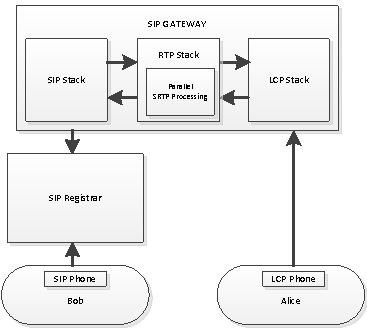
\includegraphics[width=8.5cm,keepaspectratio]{fig/scenario1.pdf}
  \label{fig:comp}
\end{figure}
\end{frame}


\frame[plain]{\bluepage{Děkuji za pozornost}}

\frame[plain]{\bluepage{}}


\begin{frame}
\frametitle{SIP Gateway}
\begin{figure}[H]
  \centering
      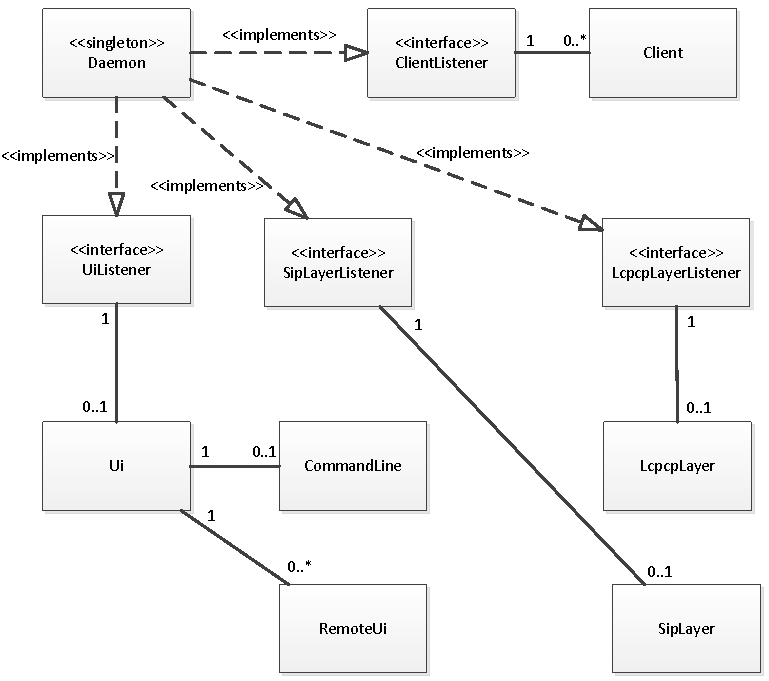
\includegraphics[width=9cm,keepaspectratio]{fig/sipgw.pdf}
  \label{fig:comp}
\end{figure}
\end{frame}


\begin{frame}
\frametitle{LCP Stack}
\begin{figure}[H]
  \centering
      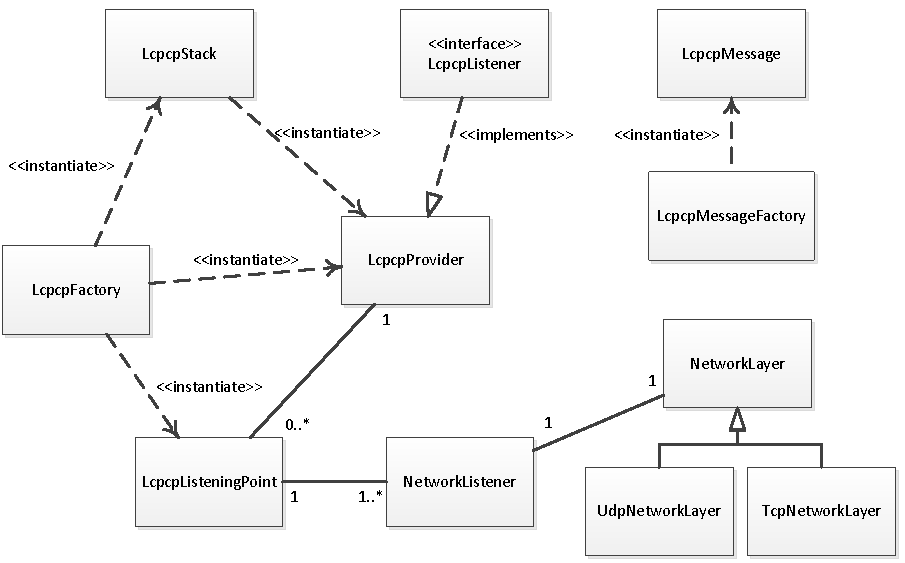
\includegraphics[width=11cm,keepaspectratio]{fig/lcpstack.pdf}
  \label{fig:comp}
\end{figure}
\end{frame}

\end{document}
